\documentclass{article}
\usepackage{tikz}
\usetikzlibrary{shapes.geometric, arrows, positioning, calc, shapes.multipart}

\begin{document}
\begin{tikzpicture}[
    node distance = 2cm,
    box/.style = {rectangle, draw, rounded corners, minimum width=2.5cm, minimum height=1cm},
    decision/.style = {diamond, draw, aspect=2, minimum width=3cm},
    database/.style = {cylinder, draw, shape border rotate=90, aspect=0.3},
    arrow/.style = {thick, ->, >=stealth}
]

% User Interface Layer
\node[box] (user) {User Interface};
\node[box, below=of user] (auth) {Authentication};
\node[decision, below=of auth] (valid) {Valid?};
\node[box, below right=of valid] (dashboard) {Dashboard};
\node[box, right=of dashboard] (balance) {Balance Display};

% Transaction Flow
\node[box, below=of dashboard] (transfer) {Transfer Module};
\node[decision, below=of transfer] (funds) {Sufficient\\ Funds?};
\node[box, below left=of funds] (reject) {Reject Transfer};
\node[box, below right=of funds] (process) {Process Transfer};
\node[database, right=of process] (transactions) {Transaction\\ History};

% Transaction Analytics (Using TikZ for Charts)
\node[box, right=of transactions] (analytics) {Analytics};
\begin{scope}[xshift=12cm, yshift=-2cm]
    % Simple Bar Chart
    \draw[thick] (0,0) -- (0,4) -- (4,4);
    \foreach \x/\h in {0.5/2, 1.5/3, 2.5/1, 3.5/2.5} {
        \fill[blue!30] (\x,0) rectangle (\x+0.4,\h);
    }
\end{scope}

% Connections
\draw[arrow] (user) -- (auth);
\draw[arrow] (auth) -- (valid);
\draw[arrow] (valid) -- node[right] {Yes} (dashboard);
\draw[arrow] (valid) -| node[above] {No} (user);
\draw[arrow] (dashboard) -- (transfer);
\draw[arrow] (dashboard) -- (balance);
\draw[arrow] (transfer) -- (funds);
\draw[arrow] (funds) -- node[left] {No} (reject);
\draw[arrow] (funds) -- node[right] {Yes} (process);
\draw[arrow] (process) -- (transactions);
\draw[arrow] (transactions) -- (analytics);

% Security Layer (represented as a background rectangle)
\begin{scope}[on background layer]
    \node[rectangle, draw=red!50, dashed, fit=(auth)(process)(transactions), 
          inner sep=1cm, label=above:Security Layer] {};
\end{scope}

\end{tikzpicture}

% Transaction Volume Visualization
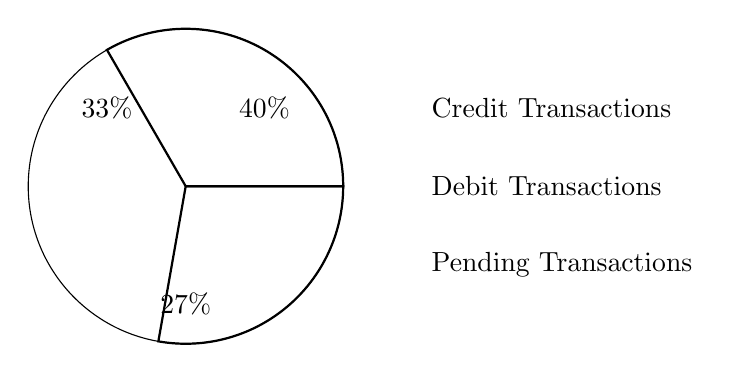
\begin{tikzpicture}[
    pie chart/.style={
        circle,
        draw,
        minimum size=4cm,
    }
]
\node[pie chart] at (0,0) {};
\draw[thick] (0,0) -- (2,0) arc(0:120:2) -- (0,0);
\draw[thick] (0,0) -- (2,0) arc(0:-100:2) -- (0,0);
\node at (1,1) {40\%};
\node at (-1,1) {33\%};
\node at (0,-1.5) {27\%};

\node[right] at (3,1) {Credit Transactions};
\node[right] at (3,0) {Debit Transactions};
\node[right] at (3,-1) {Pending Transactions};
\end{tikzpicture}

% Risk Assessment Matrix
\begin{tikzpicture}[
    matrix/.style={
        matrix of nodes,
        nodes={rectangle, draw, minimum size=1cm},
        row sep=-\pgflinewidth,
        column sep=-\pgflinewidth
    }
]
\matrix (m) [matrix] {
    High Risk & Medium Risk & Low Risk \\
    High Value & Medium Value & Low Value \\
    Priority 1 & Priority 2 & Priority 3 \\
};
\end{tikzpicture}

\end{document} 